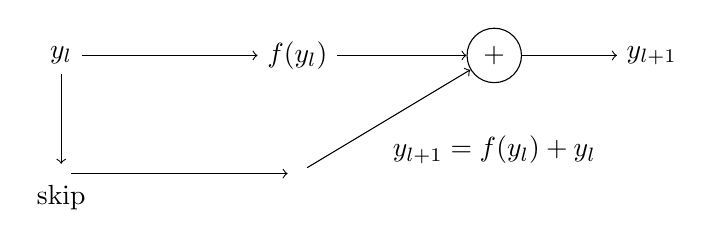
\begin{tikzpicture}[node distance=2cm, auto]
  % Input node
  \node (input) {$y_l$};
  
  % Upper path: transformation f(y_l)
  \node [right of=input, node distance=3cm] (f_block) {$f(y_l)$};
  \draw [->] (input) -- (f_block);
  
  % Lower path: skip connection
  \node [below of=input, node distance=1.5cm] (skip_start) {};
  \node [right of=skip_start, node distance=3cm] (skip_end) {};
  \draw [->] (input) -- (skip_start);
  \draw [->] (skip_start) -- (skip_end);
  \node [below of=skip_start, node distance=0.3cm] {skip};
  
  % Sum node
  \node [right of=f_block, node distance=2.5cm, circle, draw] (sum) {$+$};
  \draw [->] (f_block) -- (sum);
  \draw [->] (skip_end) -- (sum);
  
  % Output node
  \node [right of=sum, node distance=2cm] (output) {$y_{l+1}$};
  \draw [->] (sum) -- (output);
  
  % Equation label
  \node [below of=sum, node distance=1.2cm] {$y_{l+1} = f(y_l) + y_l$};
\end{tikzpicture}